\chapter{Des intégrales de chemin aux propagateurs et aux sommets}

Avant d’aborder l’inventaire des particules et de leurs interactions, il convient de clarifier la construction centrale. Un lagrangien ne se contente pas d’encoder les équations classiques des champs. Par l’intermédiaire de l’intégrale de chemin, il fournit aussi les amplitudes associées à la propagation, à la désintégration, à la fusion et à la diffusion des particules. C’est la voie la plus directe de la théorie quantique des champs aux diagrammes de Feynman.

\section{Principe de moindre action pour les particules et les champs}

L’intégrale de chemin de Feynman est le pendant quantique du principe de moindre action. Considérons d’abord une particule newtonienne ordinaire, dont le lagrangien dépend de ses coordonnées et de ses vitesses,
\begin{equation}
\mathcal{L}=\mathcal{L}(x,\dot{x}),
\end{equation}
et l’action associée à une trajectoire est
\begin{equation}
S[x]=\int \mathcal{L}(x,\dot{x})\,dt.
\end{equation}
Toute trajectoire candidate reliant deux points de l’espace-temps possède une action, qu’elle satisfasse ou non aux équations de Newton. La trajectoire classique se distingue par le fait que l’action y est stationnaire. Selon la formulation traditionnelle du ``principe de moindre action'', elle minimise l’action, bien que la stationnarité soit une affirmation plus générale. La condition de stationnarité donne les équations différentielles classiques du mouvement.

\begin{figure}[htbp]
\centering
\includegraphics[width=0.72\textwidth]{lecture_10_figure_02.png}
\caption{Intégrale d’action le long d’une trajectoire de particule.}
\lectureframe{00:02:14}
\end{figure}

La même structure s’applique à un champ classique. Désignons génériquement tous les champs par \(\phi\). La densité lagrangienne locale d’un champ peut dépendre des champs ainsi que de leurs dérivées spatiales et temporelles :
\begin{equation}
\mathcal{L}
=\mathcal{L}\!\left(\phi,\frac{\partial\phi}{\partial x^\mu}\right)
=\mathcal{L}(\phi,\partial_\mu\phi).
\end{equation}
La relativité exige que \(\mathcal{L}\) se transforme comme un scalaire de Lorentz. Sous cette condition, les combinaisons scalaires formées à partir des champs et de leurs dérivées fournissent les termes possibles du lagrangien.

\begin{figure}[htbp]
\centering
\includegraphics[width=0.62\textwidth]{lecture_10_figure_03.png}
\caption{Dépendance du lagrangien de champ à l’égard du champ et de ses dérivées d’espace-temps.}
\lectureframe{00:04:09}
\end{figure}

Pour un champ, l’action est intégrée sur une région de l’espace-temps :
\begin{equation}
S[\phi]=\int_{\Omega} d^4x\,\mathcal{L}(\phi,\partial_\mu\phi),
\qquad
d^4x=dt\,dx\,dy\,dz.
\end{equation}
L’action d’une particule s’intègre sur le temps le long d’un trajet. Celle d’un champ est l’intégrale de la densité lagrangienne sur toute une région de l’espace-temps.

L’analogue de la fixation des extrémités d’un trajet de particule consiste à prescrire la configuration complète du champ sur une tranche de temps initiale et sur une tranche de temps finale. Si le champ initial est \(\phi_{\mathrm{i}}(\mathbf{x})\) et le champ final \(\phi_{\mathrm{f}}(\mathbf{x})\), un champ interpolant remplit toute la tranche d’espace-temps comprise entre les deux. Lorsque les données aux frontières admettent une solution classique interpolante, celle-ci est un point stationnaire de l’action, les configurations aux frontières étant maintenues fixes.
\editorialnote{Deux configurations complètes arbitraires du champ sur deux tranches de temps n’admettent pas nécessairement de solution classique. L’énoncé de stationnarité de l’action se limite donc aux données aux frontières pour lesquelles il existe une solution interpolante.}

La géométrie est le pendant, pour la théorie des champs, d’un trajet de particule.\footnote{La tranche d’espace-temps est reconstituée à partir du diagramme vers 00:04:29.}
\begin{figure}[htbp]
\centering
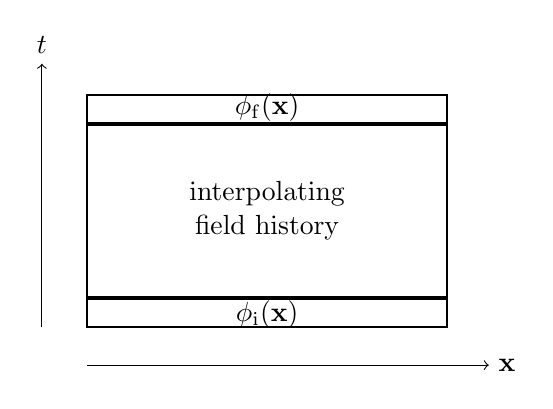
\begin{tikzpicture}[scale=0.88]
\draw[->] (-0.65,0) -- (-0.65,3.8) node[above] {$t$};
\draw[->] (0,-0.55) -- (5.8,-0.55) node[right] {$\mathbf{x}$};
\draw[thick] (0,0) rectangle (5.2,3.35);
\draw[very thick] (0,0.42) -- (5.2,0.42);
\draw[very thick] (0,2.93) -- (5.2,2.93);
\node at (2.6,0.18) {$\phi_{\mathrm{i}}(\mathbf{x})$};
\node at (2.6,3.17) {$\phi_{\mathrm{f}}(\mathbf{x})$};
\node[align=center] at (2.6,1.68) {interpolating\\field history};
\end{tikzpicture}
\caption{Configurations initiale et finale du champ délimitant une région d’espace-temps.}
\end{figure}

\begin{classroomqa}
\lecturetimestamp{00:07:34}
\audiencequestion{Un champ peut-il reprendre la même valeur ?}
\lecturerresponse{Oui. Rien n’empêche un champ de reprendre une valeur antérieure, pas plus qu’une coordonnée de particule ne peut être empêchée de reprendre une position antérieure.}
\end{classroomqa}

\begin{classroomqa}
\lecturetimestamp{00:07:46}
\audiencequestion{Pourquoi parler d’événements de l’espace-temps ou d’une trajectoire lorsque les données aux frontières sont des valeurs du champ ?}
\lecturerresponse{La trajectoire de la particule est remplacée par une histoire du champ. Chaque extrémité dans l’espace des champs correspond au champ tout entier sur une tranche de temps choisie, et une histoire spécifie le champ en chaque point de la région d’espace-temps comprise entre les deux tranches.}
\end{classroomqa}

Imposer la stationnarité de l’action au champ interpolant produit des équations aux dérivées partielles. Selon les champs et le lagrangien, on obtient notamment des équations telles que celles de Maxwell et, pour une action gravitationnelle, celles d’Einstein. Il n’est pas nécessaire de détailler ici la dérivation variationnelle ; la séquence importante est
\begin{equation}
\mathcal{L}
\longrightarrow
S[\phi]
\longrightarrow
\text{classical field equations}.
\end{equation}

\section{Somme de Feynman sur les trajectoires des particules}

En mécanique quantique, la question de savoir quelle trajectoire est suivie devient une question d’amplitudes. Imaginons qu’on injecte une particule en \((x,t)\), qu’on ferme les yeux un moment, puis qu’on active un détecteur en \((x',t')\). L’amplitude
\begin{equation}
\mathcal{A}(x,t;x',t')
\end{equation}
est un nombre complexe. Son carré en module est la probabilité :
\begin{equation}
\begin{aligned}
P(x,t;x',t')
&=\left|\mathcal{A}(x,t;x',t')\right|^2\\
&=\mathcal{A}(x,t;x',t')
\mathcal{A}(x,t;x',t')^*.
\end{aligned}
\end{equation}

La règle de Feynman associe une action à chaque trajectoire candidate et lui attribue la phase
\begin{equation}
\exp\!\left(-\frac{i}{\hbar}S[x]\right)
=
\exp\!\left[-\frac{i}{\hbar}\int \mathcal{L}(x,\dot{x})\,dt\right].
\end{equation}

\begin{figure}[htbp]
\centering
\includegraphics[width=0.70\textwidth]{lecture_10_figure_04.png}
\caption{Phase complexe associée à une trajectoire de particule.}
\lectureframe{00:11:52}
\end{figure}

Le facteur \(\hbar\) est nécessaire pour rendre l’exposant sans dimension.\footnote{À 00:11:52, ce qui est écrit au tableau se lit naturellement \(e^{-i\int\mathcal{L}\,dt}\) ; le facteur \(\hbar\) est ajouté oralement à 00:12:02.} L’amplitude de transition est la somme de ces phases sur toutes les trajectoires possibles reliant les extrémités :
\begin{equation}
\mathcal{A}(x,t;x',t')
=
\sum_{\substack{\text{paths }x(\tau)\\(x,t)\rightarrow(x',t')}}
\exp\!\left(-\frac{i}{\hbar}S[x]\right).
\end{equation}
Ici, « ``trajectoire possible'' » ne désigne pas une solution des équations de Newton, mais n’importe quelle trajectoire incluse dans la somme. En mécanique quantique non relativiste, les trajectoires avancent dans le temps ; elles ne bouclent pas en remontant le temps. La constante de Planck a les dimensions d’une action, si bien que \(S/\hbar\) est sans dimension.

L’exponentielle s’impose naturellement parce que les amplitudes associées à des petits pas successifs se multiplient. Si l’on divise une trajectoire en morceaux successifs, les actions s’additionnent,
\begin{equation}
S=S_1+S_2+\cdots,
\end{equation}
tandis que les phases se multiplient :
\begin{equation}
e^{-iS/\hbar}
=e^{-iS_1/\hbar}e^{-iS_2/\hbar}\cdots.
\end{equation}
Le facteur \(i\) n’est pas un simple artifice de calcul ; il fait partie de la règle de la mécanique quantique.

\begin{classroomqa}
\lecturetimestamp{00:13:27}
\audiencequestion{L’exponentielle est-elle liée à la multiplication des amplitudes associées à des petits pas successifs ?}
\lecturerresponse{Oui. Les amplitudes des pas successifs se multiplient, tandis que les morceaux correspondants de l’action s’additionnent.}
\end{classroomqa}

\begin{classroomqa}
\lecturetimestamp{00:13:49}
\audiencequestion{La somme sur les trajectoires est-elle elle-même la probabilité ?}
\lecturerresponse{Non. La somme sur les trajectoires est une amplitude de probabilité, généralement complexe. Son produit par son conjugué complexe donne la probabilité.}
\end{classroomqa}

\section{Somme sur les histoires de champ}

La même formulation s’étend à la théorie quantique des champs, même si la construction présentée ici restera délibérément non rigoureuse. Partons d’une configuration initiale du champ \(\phi(\mathbf{x})\) et d’une configuration finale spécifiée séparément \(\phi'(\mathbf{x})\). Ce sont des fonctions complètes de l’espace, et non des valeurs en deux points isolés.

On peut imaginer un appareil idéalisé qui prépare le champ en chaque point de l’espace, laisse le système évoluer, puis mesure le champ en tout point. Un tel appareil n’est pas réaliste, mais il pose clairement la question conceptuelle : quelle est l’amplitude de transition entre la configuration initiale complète du champ et la configuration finale ?

Toute histoire de champ interpolante imaginable contribue à la somme. Pour chaque histoire, on calcule
\begin{equation}
S[\phi]=\int d^4x\,\mathcal{L}(\phi,\partial_\mu\phi)
\end{equation}
et on lui associe la phase correspondante. Schématiquement,
\begin{equation}
\mathcal{A}\!\left[\phi(\mathbf{x})\rightarrow\phi'(\mathbf{x})\right]
=
\sum_{\substack{\text{field histories}\\
\phi_{\mathrm{i}}=\phi,\;\phi_{\mathrm{f}}=\phi'}}
\exp\!\left(-\frac{i}{\hbar}S[\phi]\right).
\end{equation}
Une histoire n’a pas besoin de satisfaire aux équations classiques du champ. C’est simplement une assignation complète de valeurs du champ dans toute la région d’espace-temps intermédiaire.

\begin{classroomqa}
\lecturetimestamp{00:17:39}
\audiencequestion{Il existe une infinité d’histoires, et chaque phase a un module égal à un. Comment leur somme peut-elle converger ? Minimise-t-on les histoires ?}
\lecturerresponse{On somme les histoires ; on ne les minimise pas. Les termes sont des phases réparties sur le cercle unité et peuvent donc s’annuler les uns les autres. C’est différent de l’addition d’une infinité de termes positifs dont les valeurs restent bornées loin de zéro. Les intégrales oscillantes peuvent converger ; la représentation de Fourier d’une fonction delta en est un exemple bien connu. Si les phases étaient réparties uniformément sur le cercle, leur somme vectorielle serait nulle. La plupart des histoires s’annulent largement entre elles. Celles qui sont proches d’une trajectoire où l’action est stationnaire s’annulent moins, car la phase y varie moins rapidement ; c’est ainsi qu’émerge la limite classique.}
\end{classroomqa}

\editorialnote{Une intégrale de chemin en temps réel nécessite en général une prescription de convergence. La discussion du cercle unité fournit ici l’argument d’annulation oscillante ; elle ne constitue pas une preuve générale de convergence.}

L’annulation peut être représentée comme une somme vectorielle dans le plan complexe.\footnote{La construction du cercle unité est reconstituée à partir de la discussion au tableau entre 00:18:32--00:20:21.}
\begin{figure}[htbp]
\centering
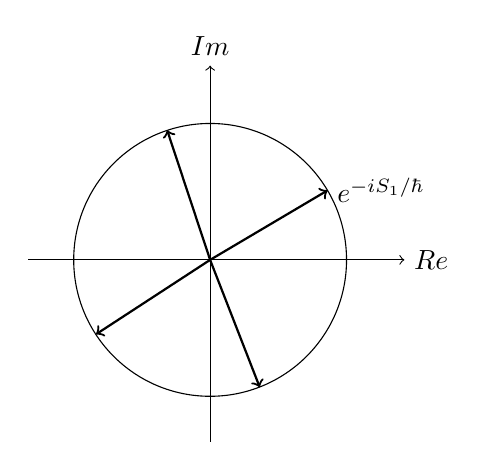
\begin{tikzpicture}[scale=1.05]
\draw[->] (-2.2,0) -- (2.35,0) node[right] {$\operatorname{Re}$};
\draw[->] (0,-2.2) -- (0,2.35) node[above] {$\operatorname{Im}$};
\draw (0,0) circle (1.65);
\draw[thick,->] (0,0) -- (1.42,0.84);
\draw[thick,->] (0,0) -- (-1.38,-0.90);
\draw[thick,->] (0,0) -- (-0.52,1.57);
\draw[thick,->] (0,0) -- (0.60,-1.54);
\node[right] at (1.42,0.84) {$e^{-iS_1/\hbar}$};
\end{tikzpicture}
\caption{Des phases de module un peuvent s’annuler lorsque leurs directions diffèrent.}
\end{figure}

En effet,
\begin{equation}
e^{-iS/\hbar}
=
\cos\!\left(\frac{S}{\hbar}\right)
-i\sin\!\left(\frac{S}{\hbar}\right).
\end{equation}
Chaque contribution est un vecteur unitaire. Des contributions orientées dans des directions différentes s’ajoutent ou se soustraient. À proximité d’un point stationnaire de \(S\), les histoires voisines ont presque la même phase et leurs contributions se renforcent donc plus efficacement. Loin de la stationnarité de l’action, la phase varie rapidement et l’interférence destructive domine.

Cette structure d’intégrale de chemin sous-tend pratiquement toute la théorie quantique des champs moderne. La prochaine étape pratique sera énoncée plutôt que dérivée. C’est une approche excessivement simplifiée du calcul, mais elle montre comment un même objet peut se prêter à deux descriptions.

Calculer un processus revient à calculer une probabilité de transition entre un état initial et un état final. Une description spécifie une configuration initiale du champ et une configuration finale. L’autre spécifie les particules incidentes et les particules sortantes, quanta d’un ou de plusieurs champs. Ces questions semblent différentes, mais on les calcule toutes deux à partir de la même intégrale de chemin de la théorie des champs.

\section{Formulation sur un espace-temps discret}

Pour donner un sens concret à la somme sur les histoires de champ, divisons l’espace-temps en petites cellules et attribuons une valeur du champ à chacune d’elles. On approche la limite du continuum en réduisant la taille des cellules, mais, pour l’instant, elles restent finies. La somme formelle sur des fonctions devient ainsi une somme sur les assignations de nombres aux cellules du réseau.

Une heuristique antérieure utilise, pour chaque cellule, un produit de facteurs ressemblant à \(1+\mathcal{L}_i\), puis identifie les termes décrivant la propagation et les collisions de particules. La construction est assez centrale pour être reprise, mais le facteur doit être corrigé. La petite quantité n’est pas le lagrangien lui-même, mais l’action contenue dans une cellule.

Si une cellule a pour volume d’espace-temps
\begin{equation}
a^4=\Delta t\,\Delta x\,\Delta y\,\Delta z,
\end{equation}
alors son action est
\begin{equation}
A_i=\mathcal{L}_i a^4.
\end{equation}
Comme la cellule est petite, \(A_i\) est petit. En omettant provisoirement \(\hbar\), le facteur élémentaire corrigé est
\begin{equation}
1-iA_i,
\end{equation}
plutôt que \(1+\mathcal{L}_i\).

Pour tout petit \(\epsilon\),
\begin{equation}
1+\epsilon\simeq e^\epsilon,
\end{equation}
car
\begin{equation}
e^\epsilon
=1+\epsilon+\frac{\epsilon^2}{2!}
+\frac{\epsilon^3}{3!}+\cdots.
\end{equation}
Ainsi, dans ces unités provisoires, \(1-iA_i\) approche \(e^{-iA_i}\) si la cellule est suffisamment petite. Il est plus simple d’utiliser dès le départ le facteur exponentiel exact.

\begin{classroomqa}
\lecturetimestamp{00:27:57}
\audiencequestion{L’exponentielle nécessite-t-elle un facteur de \(\hbar\) ?}
\lecturerresponse{Oui. Le facteur sans dimension associé à une cellule est \(1-iA_i/\hbar\) au premier ordre, et l’exponentielle exacte est \(\exp(-iA_i/\hbar)\). On peut ensuite adopter des unités telles que \(\hbar=1\).}
\end{classroomqa}

En rétablissant \(\hbar\), le facteur intermédiaire corrigé et sa forme exponentielle sont
\begin{equation}
1-\frac{i}{\hbar}A_i
\simeq
\exp\!\left(-\frac{i}{\hbar}A_i\right).
\end{equation}

Pour une histoire fixée, remplaçons l’intégrale sur l’espace-temps par une somme des actions des cellules :
\begin{equation}
S[\phi]
=\int d^4x\,\mathcal{L}
\;\longrightarrow\;
\sum_i A_i.
\end{equation}
La phase associée à cette histoire devient
\begin{equation}
\exp\!\left(-\frac{i}{\hbar}\sum_i A_i\right).
\end{equation}
Une exponentielle d’une somme est un produit d’exponentielles :
\begin{equation}
\exp\!\left(-\frac{i}{\hbar}\sum_i A_i\right)
=
\prod_i\exp\!\left(-\frac{i}{\hbar}A_i\right).
\end{equation}
L’ordre des opérations compte. On choisit d’abord une histoire complète et on multiplie les poids de ses cellules. Ce n’est qu’ensuite qu’on somme sur les différentes histoires.

Le réseau rend aussi explicites les données aux frontières.\footnote{Le damier et ses première et dernière rangées fixes sont reconstitués à partir des diagrammes vers 00:23:54 et 00:30:49.}
\begin{figure}[htbp]
\centering
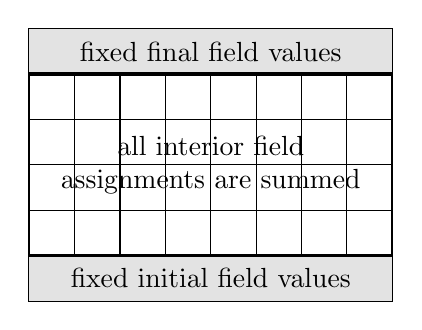
\begin{tikzpicture}[scale=0.72]
\draw[step=0.8,thin] (0,0) grid (6.4,4.8);
\draw[thick] (0,0) rectangle (6.4,4.8);
\fill[gray!22] (0,0) rectangle (6.4,0.8);
\fill[gray!22] (0,4.0) rectangle (6.4,4.8);
\draw[very thick] (0,0.8) -- (6.4,0.8);
\draw[very thick] (0,4.0) -- (6.4,4.0);
\node at (3.2,0.4) {fixed initial field values};
\node at (3.2,4.4) {fixed final field values};
\node[align=center] at (3.2,2.4) {all interior field\\assignments are summed};
\end{tikzpicture}
\caption{Histoires de champ discrètes avec rangées initiale et finale du réseau fixées.}
\end{figure}

La première rangée spécifie la configuration initiale du champ et la dernière, sa configuration finale. Chaque cellule intérieure peut prendre toutes les valeurs du champ prévues par la discrétisation. L’amplitude de transition prend donc la forme schématique
\begin{equation}
\mathcal{A}\!\left[\phi_{\mathrm{i}}\rightarrow\phi_{\mathrm{f}}\right]
=
\sum_{\{\phi\}_{\mathrm{interior}}}
\prod_i\exp\!\left(-\frac{i}{\hbar}A_i[\phi]\right),
\end{equation}
les première et dernière rangées étant maintenues fixes. De manière équivalente, pour chaque assignation intérieure, on calcule l’exponentielle de l’action totale, puis on ajoute cette contribution à celles de toutes les autres assignations.

\section{Des configurations de champ aux configurations de particules}

La même amplitude de transition peut être décrite en termes de champs ou de particules. Au lieu de fixer le champ sur les tranches de temps initiale et finale, on peut spécifier un ensemble de quanta de champ incidents et un ensemble de quanta sortants, puis chercher l’amplitude qui les relie. L’objet calculé est le même ; seule la description des frontières change.

Les champs quantiques contiennent des opérateurs de création et d’annihilation. Les produits de champs agissent donc sur les états de particules en créant, détruisant ou déplaçant des quanta. C’est cette lecture en termes d’opérateurs qui transforme l’intégrale de chemin sur réseau en un ensemble de règles pour les particules.

\begin{classroomqa}
\lecturetimestamp{00:34:11}
\audiencequestion{Les quanta de champ sont-ils nécessairement identifiables à des particules ?}
\lecturerresponse{Pas toujours au sens conventionnel de particules observables séparément. Les quarks sont, par exemple, les quanta des champs de quarks, mais le confinement empêche un quark isolé de s’échapper et d’être détecté seul. Plus généralement, il n’existe pas nécessairement de correspondance biunivoque entre les champs nommés dans une théorie et les espèces de particules qui apparaissent comme états observables au sens conventionnel. Certaines théories des champs n’admettent pas cette correspondance simple. Si l’on emploie le terme « ``particule'' » au sens large pour désigner un quantum indivisible porteur d’énergie et d’autres nombres quantiques, la distinction peut alors relever en partie de la terminologie.}
\end{classroomqa}

\editorialnote{La proposition sur le couplage faible, entre 00:35:45--00:36:08, est grammaticalement ambiguë dans la source et reste ici sans interprétation. L’affirmation sûre est que les étiquettes des champs et les espèces de particules observables au sens conventionnel ne sont pas nécessairement en correspondance biunivoque.}

La somme sur le réseau porte toujours sur les valeurs du champ. Elle ne se limite pas aux configurations ressemblant à des solutions classiques régulières.

\begin{classroomqa}
\lecturetimestamp{00:36:44}
\audiencequestion{Les histoires de champ doivent-elles être continues, ou du moins approximativement continues ?}
\lecturerresponse{Non. Sur un réseau discret, les cellules voisines portent simplement des valeurs du champ, et chaque assignation est incluse dans la somme. Rien ne limite celle-ci aux histoires approximativement continues. Les champs quantiques fluctuent fortement ; les histoires typiques ne sont pas des champs classiques réguliers.}
\end{classroomqa}

Les variables assignées indépendamment sont les champs aux sites ou aux cellules du réseau. Leurs dérivées se déduisent des différences entre les valeurs aux sites voisins.

\begin{classroomqa}
\lecturetimestamp{00:37:56}
\audiencequestion{Les champs et leurs dérivées reçoivent-ils des valeurs indépendantes ?}
\lecturerresponse{Non. On assigne des valeurs du champ aux sites. Une dérivée est ensuite reconstruite à partir de la différence entre les valeurs aux sites voisins. Plusieurs conventions de différences finies sont possibles, mais les dérivées ne sont pas des variables indépendantes supplémentaires.}
\end{classroomqa}

Ainsi, pour un espacement de réseau \(a\), on peut écrire schématiquement
\begin{equation}
\partial_\mu\phi(x)
\longrightarrow
\frac{\phi(x+a\hat\mu)-\phi(x)}{a}.
\end{equation}
L’axe des valeurs du champ peut lui-même être subdivisé en petits intervalles, ce qui laisse un ensemble dénombrable de valeurs possibles en chaque site.

\begin{classroomqa}
\lecturetimestamp{00:38:53}
\audiencequestion{Que change la présence de plusieurs champs ?}
\lecturerresponse{On assigne la valeur de chaque champ en chaque site, et la somme porte sur toutes ces assignations.}
\end{classroomqa}

Il ne faut pas confondre un champ à valeurs complexes avec une fonction analytique d’une variable complexe. L’analyticité est une condition de régularité exceptionnellement forte. Les histoires dans une intégrale de chemin sur les champs n’ont pas à la satisfaire et, en général, ne sont même pas approximativement régulières.

\begin{classroomqa}
\lecturetimestamp{00:39:07}
\audiencequestion{Si les champs prennent des valeurs complexes, celles-ci doivent-elles satisfaire aux conditions de régularité des fonctions analytiques ?}
\lecturerresponse{Non. « À valeurs complexes » ne signifie pas « analytique ». La théorie des fonctions analytiques porte sur une classe de fonctions extrêmement régulières et fortement contraintes. Les histoires de champ sommées ici n’ont pas besoin d’être des fonctions analytiques de la position ; les histoires typiques sont très irrégulières et peuvent être considérées comme fortement discontinues dans la limite du continuum.}
\end{classroomqa}

Le calcul qui en résulte semble redoutable. Même après discrétisation de l’espace-temps et des valeurs du champ, le nombre d’assignations à échantillonner peut être énorme.

\begin{classroomqa}
\lecturetimestamp{00:40:04}
\audiencequestion{Comment un ordinateur sait-il combien d’assignations du réseau échantillonner, ou à quel moment le calcul a convergé ?}
\lecturerresponse{Cette question relève de la théorie de jauge sur réseau ou, plus généralement, de la théorie quantique des champs sur réseau. C’est désormais un domaine de calcul efficace. J’ai participé tout au début à l’établissement des règles de la théorie de jauge sur réseau, mais pas aux développements informatiques ultérieurs. Il a fallu environ trois semaines pour établir les règles ; le développement des outils permettant de faire ces calculs a pris quelque chose comme trente ans. Une grande part du savoir-faire pratique est venue de la mécanique statistique, où les fonctions de partition s’obtiennent aussi en sommant sur les configurations d’un réseau---par exemple, selon qu’un site d’un cristal est occupé ou non. Déterminer si l’échantillonnage a porté sur suffisamment de configurations est une question technique. Les spécialistes savent---ou pensent savoir---quand le calcul est maîtrisé, et les calculs qui en résultent concordent avec l’expérience.}
\end{classroomqa}

Les règles conceptuelles de la théorie de jauge sur réseau ont été établies rapidement ; les outils nécessaires aux calculs ont demandé beaucoup plus de temps. Le damier n’est pas une simple analogie : il constitue aussi le point de départ d’une méthode de calcul pratique.

\section{Termes quadratiques et propagation des particules}

Revenons à l’interprétation des champs en termes d’opérateurs. Pour deux sites voisins \(x\) et \(x'\), le produit
\begin{equation}
\phi(x)\phi(x')
\end{equation}
peut, dans un élément de matrice à une particule approprié, annihiler une particule en un site et en créer une à l’autre. Dans ce secteur à une particule, on peut donc le représenter comme un saut d’un lien. C’est une interprétation du produit d’opérateurs, mais pas la seule.

Les termes responsables de tels liens sont les termes dérivés. À strictement parler, ils sont associés à une paire de sites voisins, et non à une cellule unique. Une dérivée temporelle, par exemple, devient
\begin{equation}
\partial_t\phi(t,\mathbf{x})
\longrightarrow
\frac{\phi(t+a,\mathbf{x})-\phi(t,\mathbf{x})}{a},
\end{equation}
et on traite de la même manière une dérivée spatiale le long d’un lien spatial.

\begin{classroomqa}
\lecturetimestamp{00:44:39}
\audiencequestion{Les lagrangiens considérés comportent-ils des dérivées secondes ?}
\lecturerresponse{Les théories usuelles considérées ici s’écrivent avec des dérivées premières. Leurs versions sur réseau utilisent donc des différences premières entre sites voisins.}
\end{classroomqa}

Le carré d’une différence première produit à la fois des termes portant sur un même site et un terme croisé entre sites voisins :
\begin{align}
\frac{1}{2}\bigl[\phi(x)-\phi(x')\bigr]^2
&=
\frac{1}{2}\phi(x)^2
+\frac{1}{2}\phi(x')^2
-\phi(x)\phi(x').
\end{align}
Le terme croisé peut correspondre au déplacement d’un site à l’autre. Les deux carrés portent sur un même site. Les termes dérivés quadratiques sont les termes cinétiques, et ce sont d’abord leurs termes croisés entre sites voisins qui serviront à construire la propagation.

Pour isoler la combinatoire, regroupons les produits entre sites voisins sous la forme
\begin{equation}
K=\sum_{\langle x,x'\rangle}\phi(x)\phi(x').
\end{equation}
Le facteur correspondant dans le poids de l’intégrale de chemin s’écrit schématiquement
\begin{equation}
e^{-iK}.
\end{equation}
\editorialnote{Dans ce facteur schématique sur réseau, les puissances du pas du réseau, \(\hbar\), les signes de la métrique, les constantes de normalisation et les coefficients des liens sont omis.}
Son développement est
\begin{equation}
e^{-iK}
=1-iK-\frac{1}{2!}K^2+\frac{i}{3!}K^3+\cdots,
\end{equation}
ou, en faisant apparaître les sommes sur les sites voisins,
\begin{align}
e^{-iK}
={}&1
-i\sum_{\langle x,x'\rangle}\phi(x)\phi(x')
\nonumber\\
&-\frac{1}{2!}
\sum_{\langle x,x'\rangle}
\sum_{\langle y,y'\rangle}
\phi(x)\phi(x')\phi(y)\phi(y')
+\cdots .
\end{align}
Chaque facteur sélectionne indépendamment une paire de sites voisins.

Les diagrammes de particules obéissent à une règle d’absence d’extrémités libres. Une extrémité apparente n’est admise que si la condition aux frontières insère explicitement une particule sur la tranche initiale ou en retire une sur la tranche finale. Un lien isolé à l’intérieur a des extrémités non raccordées et ne représente pas une contribution complète à la transition prescrite. Les extrémités internes des liens doivent se rejoindre.

Considérons d’abord un réseau de deux couches temporelles seulement. Si l’état initial insère une particule en \(x\) et que l’état final la retire au point voisin \(x'\), le terme du premier ordre peut relier les deux insertions aux frontières :
\begin{equation}
x\longrightarrow x',
\qquad
\mathcal{A}_{\text{one link}}\sim -i.
\end{equation}
Le coefficient \(-i\) n’est que celui du développement schématique ; les facteurs de réseau et de normalisation omis restent sous-entendus.

\begin{classroomqa}
\lecturetimestamp{00:52:16}
\audiencequestion{Le terme à un lien du premier ordre ne contribue-t-il que lorsque les sites initial et final concernés sont voisins ?}
\lecturerresponse{Oui. Ce terme sélectionne une paire de sites voisins ; il ne peut donc relier ces sites aux frontières que s’ils sont voisins. La propagation sur une plus grande distance provient des produits d’ordre supérieur.}
\end{classroomqa}

Au deuxième ordre, les deux facteurs sont sommés indépendamment sur les paires de sites voisins :
\begin{equation}
K^2
=
\sum_{\langle x,x'\rangle}
\sum_{\langle y,y'\rangle}
\phi(x)\phi(x')\phi(y)\phi(y').
\end{equation}

\begin{classroomqa}
\lecturetimestamp{00:52:40}
\audiencequestion{La seconde paire de sites voisins doit-elle être contiguë à celle sélectionnée par le premier facteur ?}
\lecturerresponse{Non. Chaque facteur sélectionne indépendamment une paire de sites voisins. Les deux paires peuvent partager un site, être complètement séparées ou même être identiques. La somme inclut toutes les possibilités.}
\end{classroomqa}

Pour une particule qui se propage sur trois couches temporelles, la sélection utile au deuxième ordre comporte un site intermédiaire commun :
\begin{equation}
\bigl[\phi(x_0)\phi(x_1)\bigr]
\bigl[\phi(x_1)\phi(x_2)\bigr],
\qquad
x_0\longrightarrow x_1\longrightarrow x_2.
\end{equation}
L’extrémité du premier lien rejoint le début du second. Seules les extrémités initiale en \(x_0\) et finale en \(x_2\) restent libres ; le terme contribue donc à la transition requise à une particule. Dans l’exponentielle schématique, son coefficient est
\begin{equation}
-\frac{1}{2!}.
\end{equation}

Les sélections peuvent aussi former des sauts séparés.\footnote{Les diagrammes de liens sont reconstitués à partir de la séquence entre 00:49:18--00:55:12.}
\begin{figure}[htbp]
\centering
\resizebox{\linewidth}{!}{%
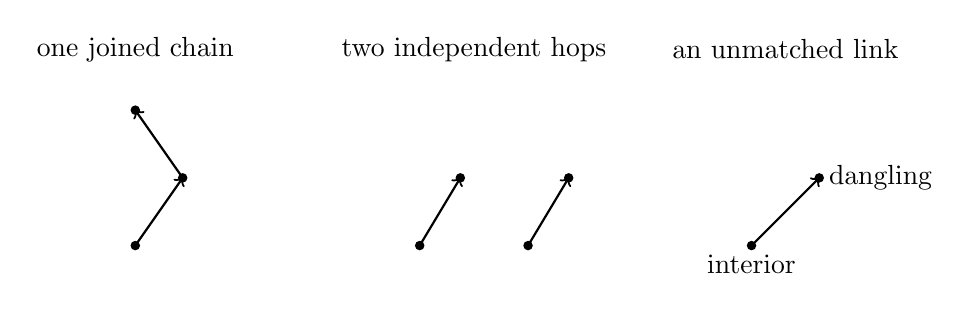
\begin{tikzpicture}[scale=0.86]
\node at (0,2.9) {one joined chain};
\fill (0,0) circle (2pt);
\fill (0.7,1.0) circle (2pt);
\fill (0,2.0) circle (2pt);
\draw[thick,->] (0,0) -- (0.7,1.0);
\draw[thick,->] (0.7,1.0) -- (0,2.0);

\begin{scope}[xshift=4.2cm]
\node at (0.8,2.9) {two independent hops};
\fill (0,0) circle (2pt);
\fill (0.6,1.0) circle (2pt);
\fill (1.6,0) circle (2pt);
\fill (2.2,1.0) circle (2pt);
\draw[thick,->] (0,0) -- (0.6,1.0);
\draw[thick,->] (1.6,0) -- (2.2,1.0);
\end{scope}

\begin{scope}[xshift=9.1cm]
\node at (0.5,2.9) {an unmatched link};
\fill (0,0) circle (2pt);
\fill (1.0,1.0) circle (2pt);
\draw[thick,->] (0,0) -- (1.0,1.0);
\node[below] at (0,0) {interior};
\node[right] at (1.0,1.0) {dangling};
\end{scope}
\end{tikzpicture}%
}
\caption{Sélections de liens voisins raccordées, indépendantes et non raccordées.}
\end{figure}

Il peut déjà y avoir plusieurs chemins à cet ordre. Pour un déplacement d’un pas temporel et d’un pas spatial sur le réseau, les deux ordres
\begin{align}
x
&\longrightarrow x+\hat t
\longrightarrow x+\hat t+\hat s,\\
x
&\longrightarrow x+\hat s
\longrightarrow x+\hat s+\hat t
\end{align}
aboutissent à la même extrémité.

\begin{classroomqa}
\lecturetimestamp{00:55:53}
\audiencequestion{Existe-t-il un autre chemin en deux étapes jusqu’à cette même extrémité diagonale ?}
\lecturerresponse{Oui. On peut effectuer d’abord le pas temporel, puis le pas spatial, ou prendre ces pas dans l’ordre inverse. Les deux chemins contribuent à la même amplitude de transition.}
\end{classroomqa}

Rien n’oblige à s’arrêter à deux liens. Le terme du troisième ordre fournit des chaînes de trois liens voisins. Un chemin peut avancer directement, faire un détour ou s’éloigner puis revenir avant d’atteindre le point final. Les ordres encore supérieurs incluent des détours plus longs et des allers-retours répétés. Le développement à tous les ordres produit donc une contribution pour chaque chemin constitué de liens locaux. L’amplitude entre deux points est la somme de tous ces chemins, avec des coefficients comportant les puissances appropriées de \(i\) et des factorielles :
\begin{equation}
\begin{gathered}
\mathcal{A}(x_{\mathrm{in}}\to x_{\mathrm{out}})
=
\sum_{\text{joined lattice routes }r}c_r,
\\
c_r\ \hbox{read from the exponential expansion}.
\end{gathered}
\end{equation}
Les coefficients sont généralement complexes, de sorte que l’amplitude qui en résulte est complexe.

La propagation relativiste ajoute une autre possibilité. Un chemin peut avancer ou reculer dans le temps et parcourir plusieurs fois le même lien.

\begin{classroomqa}
\lecturetimestamp{00:58:47}
\audiencequestion{Un chemin peut-il repasser plusieurs fois par les mêmes deux cellules ?}
\lecturerresponse{Oui. Les parcours répétés sont inclus et, dans le développement relativiste, le chemin peut aussi remonter le temps.}
\end{classroomqa}

Un segment orienté vers le passé admet deux interprétations graphiques équivalentes. On peut le considérer comme une ligne de particule qui remonte le temps. Autre possibilité : ne suivre le temps que dans le sens direct. Une paire particule--antiparticule est alors créée ; la particule poursuit son évolution vers l’avant, puis l’antiparticule rencontre la particule initiale, avec laquelle elle s’annihile. Une même ligne continue représente les deux descriptions.\footnote{Ces deux interprétations suivent le diagramme et l’explication en 00:59:00--00:59:51.}

\begin{figure}[htbp]
\centering
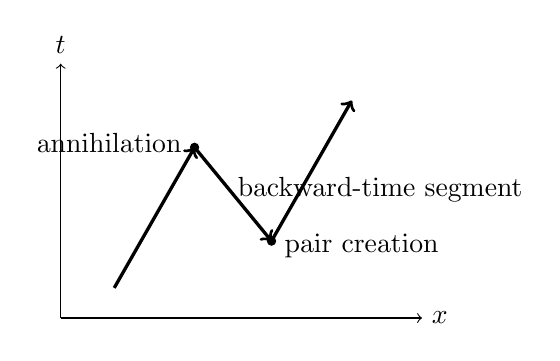
\begin{tikzpicture}[scale=0.85]
\draw[->] (0,0) -- (0,3.8) node[above] {$t$};
\draw[->] (0,0) -- (5.4,0) node[right] {$x$};
\draw[very thick,->] (0.8,0.45) -- (2.0,2.55);
\draw[very thick,->] (2.0,2.55) -- (3.15,1.15);
\draw[very thick,->] (3.15,1.15) -- (4.35,3.25);
\fill (2.0,2.55) circle (2pt);
\fill (3.15,1.15) circle (2pt);
\node[left] at (1.95,2.62) {annihilation};
\node[right] at (3.20,1.08) {pair creation};
\node[right] at (2.50,1.92) {backward-time segment};
\end{tikzpicture}
\caption{Un segment orienté vers le passé, interprété dans le sens direct comme une création de paire suivie d’une annihilation.}
\end{figure}

À grands ordres, les factorielles contrôlent la série entière de l’exponentielle, mais cela ne revient pas à contrôler la somme complète sur les configurations de champ.

\begin{classroomqa}
\lecturetimestamp{01:00:00}
\audiencequestion{Les facteurs \(1/n!\) garantissent-ils la convergence ?}
\lecturerresponse{Ils garantissent la convergence de la série de l’exponentielle pour un argument fixé. À eux seuls, ils ne garantissent pas la convergence de la somme distincte sur toutes les configurations de champ. Ce sont deux questions différentes. Sur un réseau fini, avec un ensemble fini de valeurs discrétisées du champ, le nombre de configurations est fini ; toutefois, les limites du continuum et du volume infini exigent un contrôle supplémentaire.}
\end{classroomqa}

\section{Un produit de liens, plusieurs interprétations en termes de particules}

Le produit du deuxième ordre décrit davantage que la propagation d’une seule particule. Lorsque les deux paires voisines partagent une extrémité, il peut faire avancer une particule le long d’une chaîne de deux liens :
\begin{equation}
\bigl[\phi(x_0)\phi(x_1)\bigr]
\bigl[\phi(x_1)\phi(x_2)\bigr].
\end{equation}
Lorsque les paires choisies sont disjointes, le même terme du deuxième ordre peut faire avancer deux particules, chacune d’un lien.\footnote{La comparaison entre la propagation d’une particule et deux déplacements indépendants d’un lien est reconstituée à partir de la discussion au tableau en 01:00:46--01:02:34.}
\begin{equation}
\bigl[\phi(x_0)\phi(x_1)\bigr]
\bigl[\phi(y_0)\phi(y_1)\bigr],
\qquad x_0\neq y_0.
\end{equation}
Le premier facteur transporte une particule et le second en transporte une autre. Ainsi, le développement quadratique sur réseau contient des amplitudes de propagation dans tous les secteurs à plusieurs particules. Un même ordre algébrique peut décrire un trajet connecté plus long ou plusieurs trajets disjoints plus courts.

Cela fournit beaucoup d’information, mais pas encore un véritable vertex d’interaction. Avec seulement des termes quadratiques de propagation, les lignes de particules connectées ne peuvent pas se diviser en un nombre différent de lignes. Les processus qui changent le nombre de particules nécessitent des interactions supplémentaires, même si les produits locaux d’opérateurs admettent plusieurs interprétations en termes de création et d’annihilation.

\begin{classroomqa}
\lecturetimestamp{01:03:30}
\audiencequestion{Un électron et un positron peuvent-ils s’annihiler en ne laissant aucune particule ?}
\lecturerresponse{Une contribution avec une énergie incidente non nulle et aucun état final porteur d’énergie viole la conservation de l’énergie. Lorsqu’on somme sur ses positions spatio-temporelles possibles, les amplitudes s’annulent. L’annihilation électron--positron peut se produire si un autre champ emporte l’énergie---par exemple, lorsque des quanta électromagnétiques sont produits.}
\end{classroomqa}

\editorialnote{Le passage abrégé va directement du saut quadratique à l’annihilation électron--positron. La distinction essentielle est que les termes quadratiques décrivent la propagation libre, tandis qu’une annihilation physique exige une interaction avec un autre champ ; l’amplitude sans produit final s’annule par conservation de l’énergie.}

Les termes de dérivée font donc beaucoup, mais pas tout. Les autres termes du lagrangien sont déterminés par les propriétés et les interactions des champs observées expérimentalement.

\section{Le terme de masse}

Pour un champ scalaire, la structure des dérivées considérée ici présente schématiquement la signature de signes lorentzienne
\begin{equation}
\mathcal{L}_{\mathrm{kin}}
\sim
\frac{1}{2}\left[
(\partial_t\phi)^2
-(\partial_x\phi)^2
-(\partial_y\phi)^2
-(\partial_z\phi)^2
\right].
\end{equation}
Cette expression fixe la structure temporelle moins spatiale pertinente pour la discussion ; les signes globaux et les conventions de normalisation restent implicites.

Le lagrangien peut aussi contenir des puissances du champ sans dérivée. Le terme quadratique correspondant prend la forme
\begin{equation}
\text{mass term}\ \propto\ \frac{1}{2}m^2\phi^2,
\end{equation}
où \(m^2\) est le coefficient de masse.\editorialnote{Dans ce passage, la source ne précise pas la convention de signe globale du lagrangien scalaire complet.}Dans l’interprétation schématique en termes de particules, ce terme annihile une particule puis la recrée au même site du réseau. Il ne la déplace pas. Il insère un facteur associé au même site dans un trajet :
\begin{equation}
\text{particle at }x
\longrightarrow
\boxed{m^2\phi(x)^2}
\longrightarrow
\text{particle still at }x.
\end{equation}
Chaque fois qu’une telle insertion intervient, le trajet acquiert un facteur supplémentaire proportionnel à \(m^2\).

Si l’on ne conserve que les termes de dérivée, la propagation obtenue correspond à la théorie sans masse dans ce développement schématique. Pour un champ massif, un trajet peut comporter un nombre quelconque d’insertions de masse au même site entre ses sauts. Le terme de masse modifie les poids relatifs des trajets, de sorte que le propagateur obtenu porte la masse de la particule.

\section{Termes cubiques et histoires de scission--puis de réunion}

Le terme de masse modifie le poids d’un trajet sans déplacer la particule. Les comportements plus intéressants commencent avec les termes de degré supérieur à deux. Considérons une interaction cubique,
\begin{equation}
\mathcal{L}_{\mathrm{int}}=g_3\phi^3.
\end{equation}
Dans une cellule du réseau, les trois facteurs de champ admettent quatre interprétations en termes de particules :
\begin{equation}
1\longrightarrow 2,
\qquad
2\longrightarrow 1,
\qquad
0\longrightarrow 3,
\qquad
3\longrightarrow 0.
\end{equation}
Un facteur cubique peut donc annihiler une particule et en créer deux, en annihiler deux et en créer une, en créer trois ou en annihiler trois.

Les facteurs quadratiques associés à des paires voisines assurent toujours la propagation. Une suite de ces facteurs peut amener une particule dans une cellule ; un facteur cubique situé dans cette cellule peut l’absorber et émettre deux particules ; d’autres facteurs quadratiques peuvent ensuite transporter ces deux particules au loin. Cela contribue à une amplitude avec une particule incidente et deux particules sortantes.\footnote{La géométrie du réseau est reconstituée à partir du diagramme en 01:08:48--01:09:42.}

\begin{figure}[htbp]
\centering
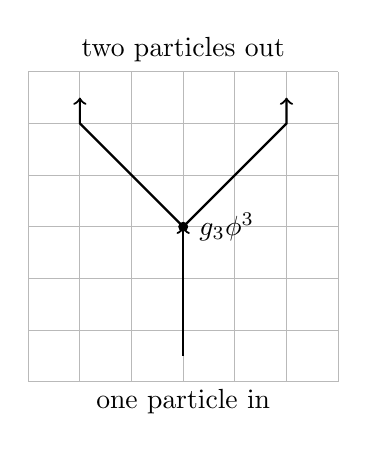
\begin{tikzpicture}[scale=0.82]
\draw[step=0.8,gray!55,thin] (0,0) grid (4.8,4.8);
\draw[thick,->] (2.4,0.4) -- (2.4,1.2) -- (2.4,2.0) -- (2.4,2.4);
\fill (2.4,2.4) circle (2.2pt);
\draw[thick,->] (2.4,2.4) -- (1.6,3.2) -- (0.8,4.0) -- (0.8,4.4);
\draw[thick,->] (2.4,2.4) -- (3.2,3.2) -- (4.0,4.0) -- (4.0,4.4);
\node[right] at (2.5,2.4) {$g_3\phi^3$};
\node at (2.4,-0.3) {one particle in};
\node at (2.4,5.15) {two particles out};
\end{tikzpicture}
\caption{Les facteurs quadratiques transportent une particule jusqu’à un vertex cubique de scission, puis l’en éloignent.}
\end{figure}

Même une amplitude où l’on trouve une seule particule à l’état initial comme à l’état final ne se réduit plus à une somme de trajets uniques et ininterrompus. Une contribution correspond à la propagation directe par une chaîne de sauts quadratiques. Une autre comporte deux facteurs cubiques : la particule se scinde en deux, qui se rejoignent ensuite. L’état intermédiaire peut donc contenir davantage de particules que l’état extérieur.\footnote{Les deux possibilités sont reconstituées à partir du diagramme en 01:09:44--01:11:36.}

\begin{figure}[htbp]
\centering
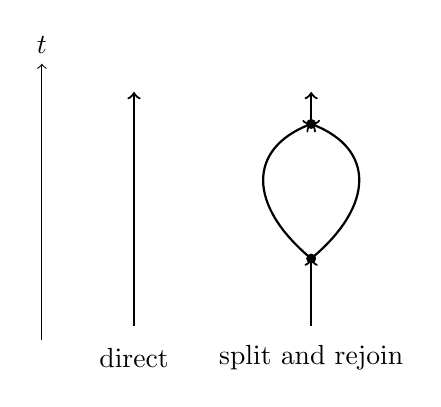
\begin{tikzpicture}[scale=0.9]
\draw[->] (-0.7,0) -- (-0.7,3.9) node[above] {$t$};
\draw[thick,->] (0.6,0.2) -- (0.6,3.5);
\node at (0.6,-0.25) {direct};
\draw[thick,->] (3.1,0.2) -- (3.1,1.15);
\fill (3.1,1.15) circle (2pt);
\draw[thick,->] (3.1,1.15) .. controls (2.2,1.9) and (2.2,2.7) .. (3.1,3.05);
\draw[thick,->] (3.1,1.15) .. controls (4.0,1.9) and (4.0,2.7) .. (3.1,3.05);
\fill (3.1,3.05) circle (2pt);
\draw[thick,->] (3.1,3.05) -- (3.1,3.5);
\node at (3.1,-0.25) {split and rejoin};
\end{tikzpicture}
\caption{Propagation directe et contribution avec scission--puis réunion pour une même amplitude à une particule.}
\end{figure}

En électrodynamique, l’exemple correspondant est celui d’un électron qui émet un photon puis le réabsorbe. Cette histoire d’émission et de réabsorption fait partie de l’amplitude de propagation de l’électron d’un point à un autre. Les ordres supérieurs comportent plusieurs émissions et absorptions. Un photon peut se convertir en une paire électron--positron, et l’électron et le positron de cette paire intermédiaire peuvent eux-mêmes échanger un photon. Rien n’impose que le contenu en particules de l’état intermédiaire soit simple au seul motif que celui des états initial et final l’est.\footnote{Les exemples de la reconstitution suivante figurent en 01:11:22--01:12:34.}

\begin{figure}[htbp]
\centering
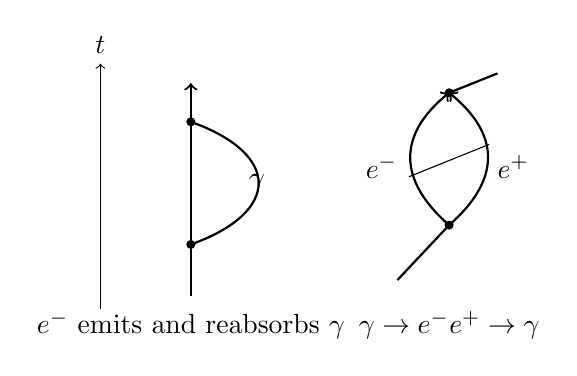
\begin{tikzpicture}[scale=0.82]
\draw[->] (-0.6,0) -- (-0.6,3.8) node[above] {$t$};
\draw[thick,->] (0.8,0.2) -- (0.8,3.5);
\fill (0.8,1.0) circle (2pt);
\fill (0.8,2.9) circle (2pt);
\draw[thick] (0.8,1.0) .. controls (2.2,1.5) and (2.2,2.4) .. (0.8,2.9);
\node[right] at (1.55,1.95) {$\gamma$};
\node at (0.8,-0.25) {$e^-$ emits and reabsorbs $\gamma$};
\draw[thick] (4.0,0.45) -- (4.8,1.3);
\fill (4.8,1.3) circle (2pt);
\draw[thick,->] (4.8,1.3) .. controls (4.0,2.0) and (4.0,2.7) .. (4.8,3.35);
\draw[thick,->] (4.8,1.3) .. controls (5.6,2.0) and (5.6,2.7) .. (4.8,3.35);
\fill (4.8,3.35) circle (2pt);
\draw[thick] (4.8,3.35) -- (5.55,3.65);
\draw[thin] (4.18,2.05) -- (5.42,2.55);
\node[left] at (4.15,2.2) {$e^-$};
\node[right] at (5.4,2.2) {$e^+$};
\node at (4.8,-0.25) {$\gamma\to e^-e^+\to\gamma$};
\end{tikzpicture}
\caption{Une contribution d’auto-émission de l’électron et une histoire de photon comportant une paire électron--positron.}
\end{figure}

Chacune de ces histoires provient d’un produit déterminé de termes dans le développement de l’exponentielle. Son coefficient comporte la puissance appropriée de \(i\), une factorielle provenant de la série de l’exponentielle et les constantes de couplage associées à ses vertex. Ce coefficient donne la contribution de cette histoire, mais l’amplitude des états initial et final spécifiés est la somme de toutes les histoires ayant ces mêmes états extérieurs.

\begin{classroomqa}
\lecturetimestamp{01:13:18}
\audiencequestion{Un même processus global peut-il se produire selon plusieurs histoires différentes, qui contribuent toutes à son amplitude ?}
\lecturerresponse{Oui. On obtient l’amplitude du processus en prenant toutes les histoires différentes qui relient le même état initial au même état final.}
\end{classroomqa}

Il existe donc deux façons équivalentes d’organiser la théorie quantique des champs. Dans la description par les champs, on spécifie une configuration de champ initiale et une configuration finale, puis on somme sur toutes les histoires du champ entre les deux. Dans la description par les particules, on décompose le champ en quanta : on spécifie le contenu en particules incidentes et sortantes, puis on somme sur toutes les histoires de particules qui les relient. Le même lagrangien gouverne les deux descriptions.

\section{Termes quartiques, lois de conservation et couplages}

Une interaction quartique,
\begin{equation}
\mathcal{L}_{\mathrm{int}}=g_4\phi^4,
\end{equation}
comporte quatre facteurs de champ en un même point. Ses interprétations locales en termes de particules incluent
\begin{equation}
\begin{gathered}
2\longrightarrow2,
\qquad
1\longrightarrow3,
\qquad
3\longrightarrow1,\\
0\longrightarrow4,
\qquad
4\longrightarrow0.
\end{gathered}
\end{equation}
Un vertex unique à quatre branches peut donc décrire une diffusion de deux particules, la scission d’une particule en trois, la réunion de trois particules en une, ou les quatre branches orientées vers l’extérieur ou vers l’intérieur.\footnote{Les orientations sont reconstituées à partir du diagramme en 01:14:28--01:15:18.}

\begin{figure}[htbp]
\centering
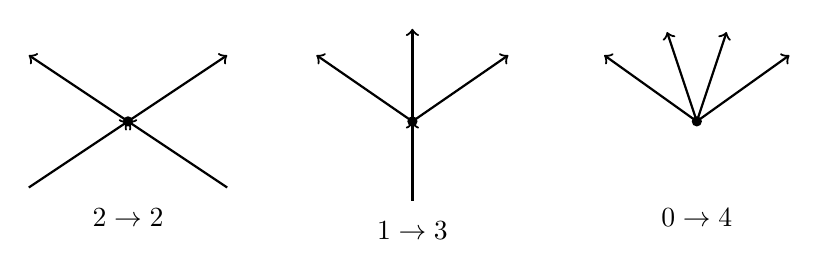
\begin{tikzpicture}[scale=0.84]
\fill (0,0) circle (2.2pt);
\draw[thick,->] (-1.5,-1.0) -- (0,0);
\draw[thick,->] (1.5,-1.0) -- (0,0);
\draw[thick,->] (0,0) -- (-1.5,1.0);
\draw[thick,->] (0,0) -- (1.5,1.0);
\node at (0,-1.45) {$2\to2$};
\begin{scope}[xshift=4.3cm]
\fill (0,0) circle (2.2pt);
\draw[thick,->] (0,-1.2) -- (0,0);
\draw[thick,->] (0,0) -- (-1.45,1.0);
\draw[thick,->] (0,0) -- (0,1.4);
\draw[thick,->] (0,0) -- (1.45,1.0);
\node at (0,-1.65) {$1\to3$};
\end{scope}
\begin{scope}[xshift=8.6cm]
\fill (0,0) circle (2.2pt);
\draw[thick,->] (0,0) -- (-1.4,1.0);
\draw[thick,->] (0,0) -- (-0.45,1.35);
\draw[thick,->] (0,0) -- (0.45,1.35);
\draw[thick,->] (0,0) -- (1.4,1.0);
\node at (0,-1.45) {$0\to4$};
\end{scope}
\end{tikzpicture}
\caption{Trois orientations locales d’un vertex d’interaction à quatre branches.}
\end{figure}

L’interprétation locale \(0\to4\) n’implique pas, à elle seule, que quatre particules puissent apparaître dans l’état final par un processus physique issu du vide. Il faut encore sommer le vertex sur toutes les positions spatio-temporelles possibles. Lorsque l’état extérieur envisagé ne peut respecter la conservation de l’énergie, les phases associées à ces positions s’annulent.

\begin{classroomqa}
\lecturetimestamp{01:15:18}
\audiencequestion{L’orientation à quatre branches sortantes décrit-elle l’apparition spontanée de quatre particules dans l’état final ?}
\lecturerresponse{C’est l’une des interprétations locales de l’opérateur à quatre champs, mais un processus sans énergie incidente viole la conservation de l’énergie. Lorsqu’on additionne les amplitudes correspondant à toutes les positions spatio-temporelles possibles du vertex, elles s’annulent.}
\end{classroomqa}

\begin{classroomqa}
\lecturetimestamp{01:15:58}
\audiencequestion{La conservation de l’énergie et celle de la quantité de mouvement résultent-elles du calcul lui-même ?}
\lecturerresponse{Oui. L’intégration du vertex sur tout le temps impose la conservation de l’énergie, et son intégration sur tout l’espace impose celle de la quantité de mouvement. La somme sur les positions du vertex s’annule si l’une ou l’autre n’est pas respectée.}
\end{classroomqa}

Sous réserve de ces lois de conservation, tout graphe autorisé par le lagrangien contribue par une certaine amplitude. La taille de cette contribution dépend notamment du coefficient de chaque terme d’interaction. Notons \(G_3\) et \(G_4\) les coefficients cubique et quartique. Chaque vertex à trois branches apporte un facteur \(G_3\), et chaque vertex à quatre branches, un facteur \(G_4\). Un graphe comportant \(V_3\) vertex cubiques et \(V_4\) vertex quartiques présente donc schématiquement la dépendance en couplages
\begin{equation}
\mathcal{A}_{\mathrm{graph}}
\propto G_3^{V_3}G_4^{V_4}.
\end{equation}

Si ces couplages sont faibles, un graphe avec peu de vertex contribue généralement davantage qu’un graphe qui en comporte beaucoup. Chaque vertex supplémentaire apporte un nouveau petit facteur. La somme perturbative peut ainsi être utile : on commence par les graphes les plus simples, puis on ajoute successivement des corrections de plus en plus faibles.

La question de savoir si la série complète converge réellement est difficile. De faibles couplages rendent plausible l’ordonnancement des contributions, mais ne règlent pas à eux seuls tous les problèmes de convergence. À fort couplage, la série naïve peut échouer complètement. Cet échec ne montre pas que la théorie sous-jacente est erronée ; il peut simplement indiquer qu’un développement en puissances du couplage était une mauvaise méthode de calcul. Les méthodes examinées ici sont surtout utiles lorsque les couplages sont assez faibles pour qu’un graphe à quatre vertex contribue bien moins qu’un graphe à deux vertex.

\begin{classroomqa}
\lecturetimestamp{01:19:24}
\audiencequestion{La théorie de la couleur peut-elle être traitée de la même façon ?}
\lecturerresponse{Oui. La théorie de la couleur peut être formulée de la même façon et sera abordée plus tard.}
\end{classroomqa}

\section{Propagateurs, vertex et descriptions complémentaires}

L’étape suivante consiste à dresser la liste des particules et à encoder leur dynamique soit dans un lagrangien, soit dans des règles de Feynman. Ces deux formes contiennent la même information. Les termes quadratiques décrivent la propagation d’un point à un autre. La ligne qui représente cette propagation s’appelle un propagateur. Les termes faisant intervenir trois champs ou davantage décrivent les endroits où des lignes se rejoignent. Ces points de rencontre sont des vertex. Par exemple,
\begin{equation}
\begin{aligned}
\text{quadratic term}
&\longleftrightarrow \text{propagator},\\
G_3\phi^3
&\longleftrightarrow \text{three-leg vertex}.
\end{aligned}
\end{equation}

On peut spécifier une théorie en attribuant un champ quantique à chaque particule et en écrivant un lagrangien qui contient toutes leurs masses et interactions. De façon équivalente, on peut énumérer tous les propagateurs, tous les vertex autorisés et le coefficient associé à chacun. L’une ou l’autre de ces listes indique quels processus sont possibles et comment attribuer des amplitudes à leurs graphes.

Par exemple, deux électrons peuvent diffuser en échangeant un photon. Chaque ligne d’électron comporte un vertex électron--électron--photon, et le propagateur du photon relie les deux vertex.\footnote{Le diagramme est reconstitué à partir de l’exemple en 01:21:38.}

\begin{figure}[htbp]
\centering
\begin{tikzpicture}[scale=0.95]
\draw[->] (-0.6,-0.2) -- (0.2,1.4);
\draw[->] (0.2,1.4) -- (-0.7,3.1);
\draw[->] (3.5,-0.2) -- (2.7,1.4);
\draw[->] (2.7,1.4) -- (3.6,3.1);
\fill (0.2,1.4) circle (2pt);
\fill (2.7,1.4) circle (2pt);
\draw[thick] (0.2,1.4) -- (2.7,1.4);
\node[above] at (1.45,1.4) {$\gamma$};
\node[left] at (-0.2,0.5) {$e^-$};
\node[right] at (3.1,0.5) {$e^-$};
\end{tikzpicture}
\caption{Diffusion de deux électrons par échange d’un photon.}
\end{figure}

Le lagrangien détermine l’amplitude de ce graphe et contient les symétries et les lois de conservation qui la contraignent. Dans un dessin orienté selon le temps, les particules placées en bas forment la configuration initiale et celles du haut, la configuration finale.

\begin{classroomqa}
\lecturetimestamp{01:22:06}
\audiencequestion{Dans un diagramme de Feynman, les particules du bas constituent-elles la configuration initiale et celles du haut la configuration finale ?}
\lecturerresponse{Oui. En bas se trouve la configuration initiale des particules, et en haut leur configuration finale.}
\end{classroomqa}

La description par les particules et celle par les champs sont complémentaires, tout comme les descriptions en termes de quantité de mouvement et de position le sont en mécanique quantique ordinaire. Elles décrivent le même système dans des bases différentes. Il existe aussi une incertitude correspondante : si le nombre de particules est spécifié avec précision, la valeur du champ est incertaine ; si la valeur du champ est spécifiée avec précision, le nombre de particules est incertain. Aucune description ne remplace l’autre, et le lagrangien est utile dans les deux.

\begin{classroomqa}
\lecturetimestamp{01:23:26}
\audiencequestion{Les constantes de couplage sont-elles prédites par la théorie ou déterminées expérimentalement ?}
\lecturerresponse{Les symétries peuvent parfois relier une constante de couplage à une autre, mais leurs valeurs numériques proviennent généralement de l’expérience.}
\end{classroomqa}

\section{Données expérimentales et prédictions d’ensemble}

La théorie quantique des champs possède en elle-même de l’élégance et de la beauté. Mais dès qu’on commence à dresser la liste des faits---les particules existantes, leurs masses et leurs constantes de couplage---, on obtient un véritable désordre. Un désordre très laid, qui ne présente guère de cohérence en dehors de celle que lui confèrent les symétries. Celles-ci relient différents types de particules et leurs processus, mais dans une mesure limitée. Une grande partie de l’inventaire reste un vaste ensemble de faits relativement disparates au sujet d’un assortiment de types de particules dont la présence semble quelque peu dépourvue de motivation.

\begin{classroomqa}
\lecturetimestamp{01:24:58}
\audiencequestion{Pourquoi peut-on se fier avec autant d’assurance aux constantes de couplage mesurées ?}
\lecturerresponse{Une fois une constante de couplage mesurée, la modifier conduit à des prédictions erronées. Sa valeur est mise à l’épreuve par les nombreux calculs qui l’utilisent.}
\end{classroomqa}

Il y a trop de particules, donc trop de champs---trop pour satisfaire un quelconque sens esthétique. On en compte de l’ordre d’une centaine. Il y a de nombreuses constantes de couplage, plus ou moins des nombres tirés de l’expérience, et de nombreuses masses qui couvrent une très large gamme de valeurs. Quelques relations les lient, mais elles sont peu nombreuses.

Mais une fois qu’on les connaît, on peut commencer à calculer. À partir de là, on peut calculer avec une grande précision tout ce qui concerne ces particules. Tout ce qui concerne les quarks, les électrons, les photons et les autres particules touche à la physique atomique, à la physique des particules, à la physique nucléaire, à la chimie et peut-être à la biologie. Les données d’entrée sont peut-être plus nombreuses qu’on ne le souhaiterait, mais la quantité de résultats est immense.

\section{L’électrodynamique quantique comme exemple perturbatif}

L’électrodynamique quantique fournit un exemple concret du développement en couplage.

\begin{classroomqa}
\lecturetimestamp{01:26:12}
\audiencequestion{Pour les électrons et les photons, combien existe-t-il de couplages d’interaction de type \(G_n\) ?}
\lecturerresponse{Il existe un seul couplage d’interaction élémentaire : la charge électrique \(e\). C’est un coefficient de type \(G_3\) associé à un vertex où un électron entre, un électron sort, et un photon est émis ou absorbé.}
\end{classroomqa}

En laissant de côté les matrices et les indices des spineurs, le contenu schématique en champs de l’interaction est
\begin{equation}
\mathcal{L}_{\mathrm{QED,int}}
\sim e\,(\text{electron bilinear})\,A,
\end{equation}
où \(A\) désigne le champ du photon. La structure détaillée en matrices de Dirac n’est pas nécessaire pour le dénombrement. La règle élémentaire de l’électrodynamique quantique décrit l’émission ou l’absorption d’un photon par un électron ; tous les graphes plus compliqués de cette théorie sont assemblés en répétant ce vertex unique.\footnote{Le vertex schématique est reconstitué à partir de 01:26:42 ; la source omet délibérément la structure détaillée en matrices.}

\begin{figure}[htbp]
\centering
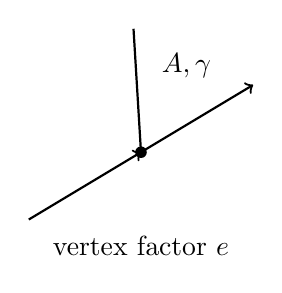
\begin{tikzpicture}[scale=0.95]
\draw[thick,->] (-1.5,-0.9) -- (0,0);
\draw[thick,->] (0,0) -- (1.5,0.9);
\draw[thick] (0,0) -- (-0.1,1.65);
\fill (0,0) circle (2.2pt);
\node[right] at (0.15,1.15) {$A,\gamma$};
\node at (0,-1.25) {vertex factor $e$};
\end{tikzpicture}
\caption{Le vertex élémentaire électron--électron--photon de l’électrodynamique quantique.}
\end{figure}

\begin{classroomqa}
\lecturetimestamp{01:27:38}
\audiencequestion{Et qu’en est-il de la diffusion électron--proton ?}
\lecturerresponse{Dans le traitement élémentaire de l’atome, on peut idéaliser le proton comme une source ponctuelle fixe, de masse infinie---une particule lourde clouée sur place. Sa propre dynamique de champ quantique n’intervient que lorsqu’on inclut la structure interne des protons et des neutrons.}
\end{classroomqa}

\begin{classroomqa}
\lecturetimestamp{01:28:30}
\audiencequestion{L’électron peut-il se déplacer à une vitesse proche de celle de la lumière par rapport à ce proton ?}
\lecturerresponse{Oui.}
\end{classroomqa}

Considérons la diffusion d’un photon par un électron. À l’ordre le plus bas, le graphe comporte deux vertex électron--électron--photon. L’amplitude est donc proportionnelle à \(e^2\) :
\begin{equation}
\mathcal{A}_{\mathrm{lowest}}\propto e^2.
\end{equation}
La probabilité, ou de façon équivalente la dépendance en couplage de la section efficace, provient du carré du module et est proportionnelle à \(e^4\) :
\begin{equation}
P_{\mathrm{lowest}}\ \text{or}\ \sigma_{\mathrm{lowest}}
\propto e^4.
\end{equation}
Avec la normalisation sans dimension conventionnelle, le couplage électrique est faible ; une véritable diffusion est donc bien moins probable que le simple passage du photon sans diffusion.

Il y a déjà deux graphes à cet ordre. Dans un premier ordre temporel, le photon incident est absorbé, puis le photon sortant est émis. Dans l’autre, le photon sortant est émis avant l’absorption du photon incident. Les deux amplitudes contribuent.\footnote{Les deux ordres temporels sont reconstitués à partir des diagrammes en 01:28:42 et 01:30:18.}

\begin{figure}[htbp]
\centering
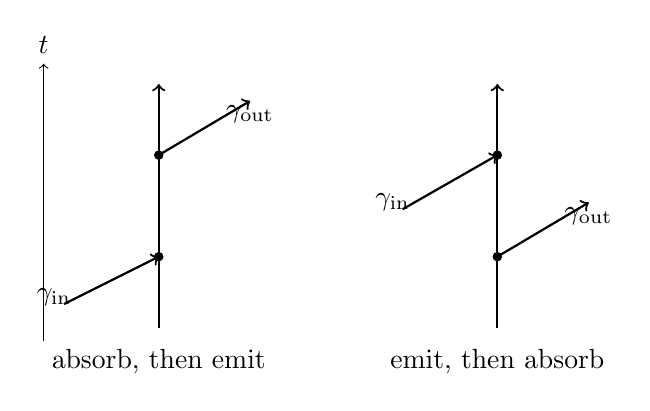
\begin{tikzpicture}[scale=0.86]
\draw[->] (-0.7,0) -- (-0.7,4.1) node[above] {$t$};
\draw[thick,->] (1.0,0.2) -- (1.0,3.8);
\fill (1.0,1.25) circle (2pt);
\fill (1.0,2.75) circle (2pt);
\draw[thick,->] (-0.4,0.55) -- (1.0,1.25);
\draw[thick,->] (1.0,2.75) -- (2.35,3.55);
\node[left] at (-0.15,0.65) {$\gamma_{\mathrm{in}}$};
\node[right] at (1.85,3.35) {$\gamma_{\mathrm{out}}$};
\node at (1.0,-0.3) {absorb, then emit};
\begin{scope}[xshift=5.0cm]
\draw[thick,->] (1.0,0.2) -- (1.0,3.8);
\fill (1.0,1.25) circle (2pt);
\fill (1.0,2.75) circle (2pt);
\draw[thick,->] (1.0,1.25) -- (2.35,2.05);
\draw[thick,->] (-0.4,1.95) -- (1.0,2.75);
\node[right] at (1.85,1.85) {$\gamma_{\mathrm{out}}$};
\node[left] at (-0.15,2.05) {$\gamma_{\mathrm{in}}$};
\node at (1.0,-0.3) {emit, then absorb};
\end{scope}
\end{tikzpicture}
\caption{Les deux ordres temporels de plus bas ordre pour la diffusion électron--photon.}
\end{figure}

L’amplitude de plus bas ordre n’est donc pas celle d’un seul graphe, mais la somme des deux :
\begin{equation}
\begin{aligned}
\mathcal{A}^{(2)}
&=
\mathcal{A}_{\mathrm{absorb\ then\ emit}}
+\mathcal{A}_{\mathrm{emit\ then\ absorb}},\\
\mathcal{A}^{(2)}&\propto e^2.
\end{aligned}
\end{equation}

Les corrections d’ordre supérieur ajoutent des vertex élémentaires. Un photon interne supplémentaire, attaché deux fois à la ligne de l’électron, ajoute deux facteurs \(e\) ; sa contribution est proportionnelle à \(e^4\) dans l’amplitude et à \(e^8\) dans son carré du module. Une ligne de photon peut aussi comporter une insertion électron--positron, qui ajoute à nouveau des vertex élémentaires et des puissances supplémentaires de \(e\). Ce ne sont que des exemples, pas une liste exhaustive ; le photon supplémentaire peut être attaché en de nombreux endroits.\footnote{Les structures d’ordre supérieur sont reconstituées à partir de 01:30:38--01:31:16.}

\begin{figure}[htbp]
\centering
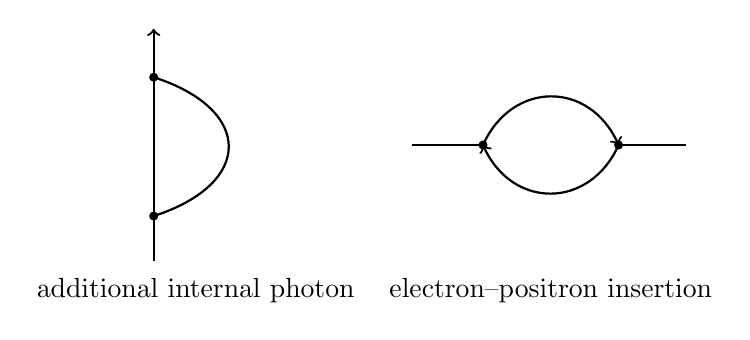
\begin{tikzpicture}[scale=0.82]
\draw[thick,->] (0.9,0.2) -- (0.9,3.8);
\fill (0.9,0.9) circle (2pt);
\fill (0.9,3.05) circle (2pt);
\draw[thick] (0.9,0.9) .. controls (2.45,1.4) and (2.45,2.55) .. (0.9,3.05);
\node at (1.55,-0.25) {additional internal photon};
\begin{scope}[xshift=5.1cm]
\draw[thick] (-0.2,2.0) -- (0.9,2.0);
\fill (0.9,2.0) circle (2pt);
\fill (3.0,2.0) circle (2pt);
\draw[thick,->] (0.9,2.0) .. controls (1.35,3.0) and (2.55,3.0) .. (3.0,2.0);
\draw[thick,->] (3.0,2.0) .. controls (2.55,1.0) and (1.35,1.0) .. (0.9,2.0);
\draw[thick] (3.0,2.0) -- (4.05,2.0);
\node at (1.95,-0.25) {electron--positron insertion};
\end{scope}
\end{tikzpicture}
\caption{Deux structures d’ordre supérieur de l’électrodynamique quantique, qui ajoutent des vertex élémentaires et des puissances supplémentaires de \(e\).}
\end{figure}

Le développement de l’électrodynamique quantique procède donc par puissances successives de \(e^2\). Chaque complication nouvelle de même ordre ajoute deux puissances de la charge électrique à l’amplitude. Avec la normalisation utilisée ici, la correction est ainsi environ cent ou deux cents fois plus faible en amplitude que l’ordre précédent. Les graphes les plus compliqués contribuent de moins en moins, ce qui peut rendre la somme perturbative utile.

On n’obtient pas la probabilité en calculant séparément le carré de chaque graphe, puis en additionnant ces carrés. Il faut d’abord additionner toutes les amplitudes qui contribuent au même processus extérieur :
\begin{equation}
\mathcal{A}_{\mathrm{total}}=\sum_r\mathcal{A}_r.
\end{equation}
Ce n’est qu’ensuite qu’on calcule
\begin{equation}
P=\left|\mathcal{A}_{\mathrm{total}}\right|^2
=\left|\sum_r\mathcal{A}_r\right|^2.
\end{equation}
Les termes croisés entre graphes différents sont des termes d’interférence. La règle est simple et essentielle : additionner d’abord, puis élever au carré.

\section{Vers l’inventaire des particules et le Modèle standard}

Une fois introduits les propagateurs, les vertex, le dénombrement des couplages et l’interférence, la description de la physique des particules peut véritablement commencer. On peut nommer les particules, préciser leurs masses, écrire les lagrangiens qui les gouvernent en s’appuyant en partie sur la théorie et en partie sur l’expérience, et étudier directement leurs symétries dans ces lagrangiens. Le même cadre mène ensuite au Modèle standard et à ses propriétés.

\begin{classroomqa}
\lecturetimestamp{01:33:22}
\audiencequestion{Peut-on remplacer le coefficient de masse constant \(m^2\) par le champ de Higgs ?}
\lecturerresponse{Oui. C’est la bonne idée, et le mécanisme sera étudié plus tard.}
\end{classroomqa}

\begin{classroomqa}
\lecturetimestamp{01:33:42}
\audiencequestion{Les points voisins du réseau \(x\) et \(x'\) peuvent-ils correspondre à deux temps différents ?}
\lecturerresponse{Oui. Ils peuvent être voisins dans la direction temporelle ; c’est ainsi que l’on représente la propagation verticale sur le réseau.}
\end{classroomqa}

Pour des points voisins, le carré de la différence finie contient à la fois des termes au même site et des termes reliant les sites :
\begin{equation}
\bigl[\phi(x)-\phi(x')\bigr]^2
=
\phi(x)^2+\phi(x')^2-2\phi(x)\phi(x').
\end{equation}

\begin{classroomqa}
\lecturetimestamp{01:33:56}
\audiencequestion{Quel terme représente une particule simplement immobile ?}
\lecturerresponse{Dans le carré de la différence finie, les termes au même site \(\phi(x)^2\) et \(\phi(x')^2\) représentent l’immobilité, tandis que le terme croisé \(\phi(x)\phi(x')\) fournit l’interprétation en termes de mouvement. Le terme de masse explicite contribue lui aussi par des facteurs associés au même site et à l’immobilité.}
\end{classroomqa}
